\documentclass[12pt]{article}
\usepackage{latexsym,tikz}
\usepackage{amssymb,amsmath}
\usepackage{graphicx}
%\usepackage{color}
\usepackage{epstopdf}


\topmargin = 0.1in \textwidth=5.7in \textheight=8.6in

\oddsidemargin = 0.2in \evensidemargin = 0.2in

\begin{document}

\begin{center}
COMPUTER SCIENCE 20, SPRING 2014 \\

\smallskip

Module \#20 (Graph Connectivity)
\end{center}
Author: Keenan Monks\\
Reviewer: Paul Handorff\\
Last modified: March 19, 2014

\medskip

\paragraph*{Executive Summary}
\begin{enumerate}

\item Connected. Two vertices are \emph{connected} if there is a path between them. \emph{Being connected} is an equivalence relation. A \emph{connected component} is a subgraph consisting of some vertex and all other vertices and edges connected to it. A graph is \emph{connected} if it has only one connected component. 

\item Edge connectivity. The edge connectivity of a graph is the smallest number of edges that must be removed to make it \emph{disconnected}. An edge whose deletion increases the number of connected components is called a \emph{bridge}.   

\item Vertex connectivity. The vertex connectivity of a graph is the smallest number of vertices that must be removed to make it \emph{disconnected}. A vertex whose deletion increases the number of connected components is called an \emph{articulation point}.
\end{enumerate}

\paragraph*{Small group problems}

\begin{enumerate}

\item What are the edge and vertex connectivities of the following graphs? 
\begin{enumerate}
\item The complete graph $K_n$.
\item A cycle of length $n$, $C_n$.
\item A path of length $n$ ($n$ vertices), $P_n$.
\item The complete bipartite graph $K_{n,n}$ (all possible edges are present).
\end{enumerate}

\item Schedule the final exams for the 6 courses --- CS50, MATH22, CS20, CS179, STAT110, and CS121 --- using the fewest number of different time slots. Courses that have students in common cannot be scheduled at the same time, and the following 8 pairs share at least one student: 

(CS50, MATH22), (CS50, CS179), (MATH22, CS20), (MATH22, STAT110), (CS20, CS179),(CS20, STAT110), (CS121, CS179), (STAT110, CS121)
\pagebreak
\item 
Below is a graph of some cities and the roads connecting them showing the maximum number of inches of snow that can fall before the roads become impassable. For example, if 2 inches of snow fall, the New York to Albany route remains operational, but if 2.25 inches of snow fall, the road is closed.


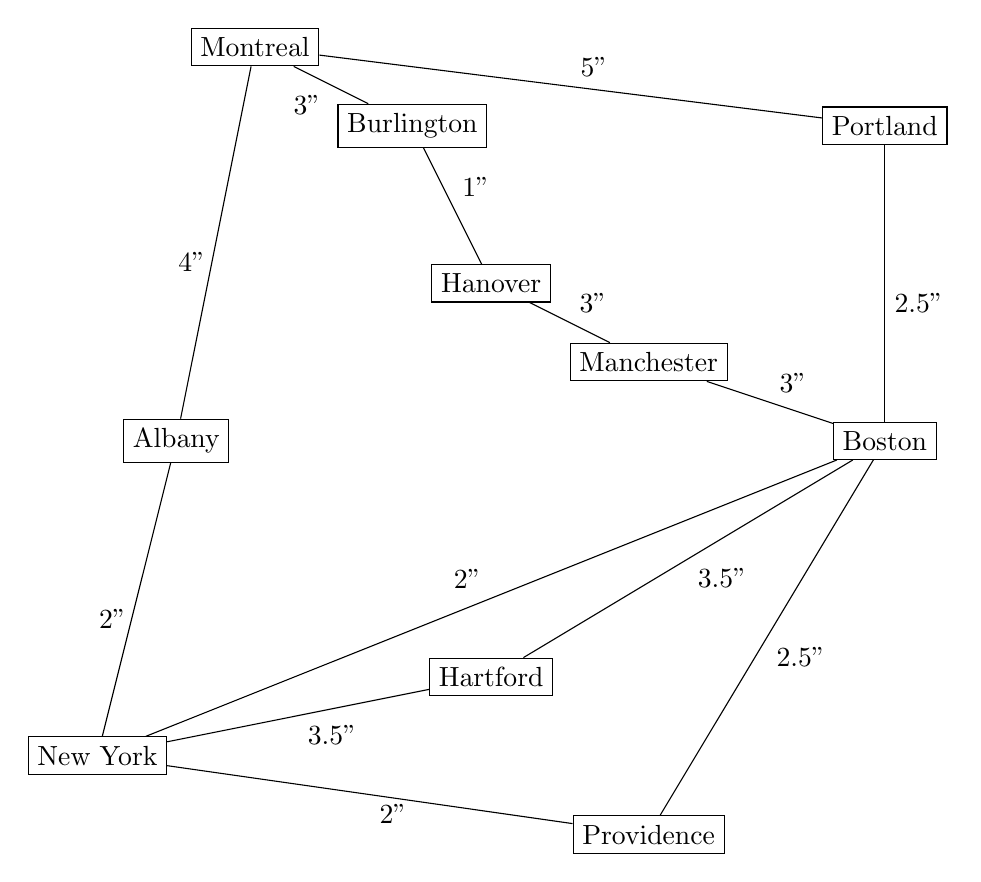
\begin{tikzpicture}
\node (New York) at (-2,0) [shape = rectangle, draw] {New York};

\node (Hartford) at (3, 1) [shape = rectangle, draw] {Hartford};

\node (Providence) at (5, -1) [shape=rectangle, draw] {Providence};

\node (Albany) at (-1,4) [shape=rectangle, draw] {Albany};

\node (Boston) at (8,4) [shape = rectangle, draw] {Boston};

\node (Manchester) at (5,5) [shape=rectangle, draw] {Manchester};

\node (Hanover) at (3, 6) [shape=rectangle, draw] {Hanover};

\node (Burlington) at (2, 8) [shape=rectangle, draw] {Burlington};

\node (Montreal) at (0,9) [shape=rectangle, draw] {Montreal};

\node (Portland) at (8,8) [shape=rectangle, draw] {Portland};


\path [-] 	(New York)	edge		node[below left]	{2''}	(Albany)
				edge		node[above left]	{2''}	(Boston)
				edge		node[below right]	{3.5''}	(Hartford)
				edge		node[below right]	{2''}	(Providence)

		(Boston)	edge		node[below right]	{2.5''}	(Portland)
				edge		node[above right]	{3''}	(Manchester)
				edge		node[below right]	{3.5''}	(Hartford)
				edge		node[below right]	{2.5''}	(Providence)

		(Montreal)	edge		node[below left]	{3''}	(Burlington)
				edge		node[below left]	{4''}	(Albany)
				edge		node[above right]	{5''}	(Portland)
		
		(Hanover)	edge		node[above right]	{1''}	(Burlington)
				edge		node[above right]	{3''}	(Manchester);
\end{tikzpicture}

\begin{enumerate}
\item Ignoring the inch labels, what is the edge connectivity of the region? What is the vertex connectivity?

\item Now following the snowfall criterion for edge removal, what is the minimum amount of snowfall that would disconnect the region?

\item Does the graph have any articulation points? Does it have any bridges? How would your answers change if 2 inches of snow fell on the region?


\end{enumerate}

\end{enumerate}

\end{document}
